\documentclass{standalone}

% Required package
\usepackage{tikz}
\usetikzlibrary{shapes, arrows.meta, positioning}

\begin{document}

\begin{tikzpicture}

\node [
	align=left] (paper) 
	at (0, 0) 
	{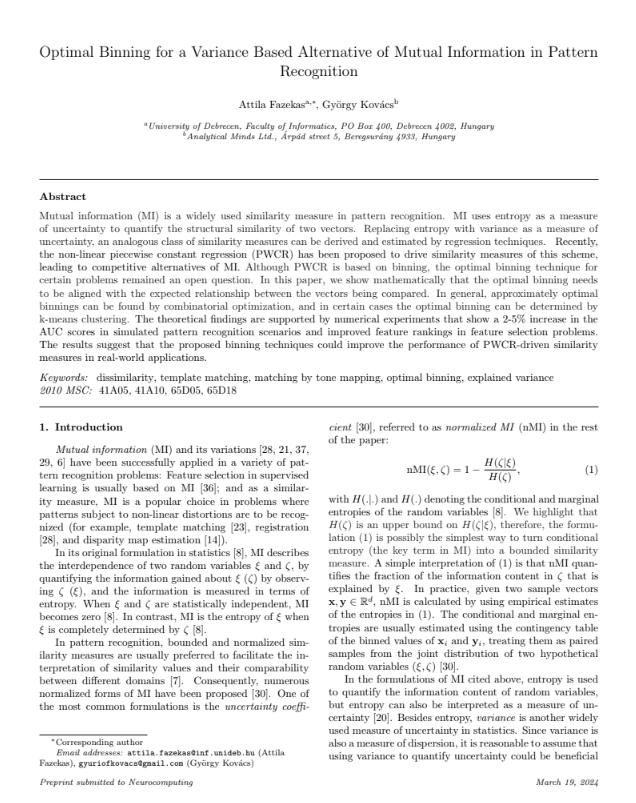
\includegraphics[width=4cm]{paper.png}};

\node [align=left] at (0, 4) {Research with binary\\ classification};
\node [align=left] at (7, 4) {Manual extraction of\\ specifics};
\node [align=left] at (17, 4) {Consistency testing};
\draw [dashed] (3.5, -3.2) -- (3.5, 4.5);
\draw [dashed] (10.5, -3.2) -- (10.5, 4.5);

% draw rectangle node
	\node[draw,
		minimum width=5cm,
		minimum height=1cm,
        align=left] (experiment) at (7,2) {Experiment\\(e.g. $p=20$, $n=300$)};
    
    \node[draw,
		minimum width=5cm,
		minimum height=1cm,
        align=left] (scores) at (7,0) {Reported scores\\(e.g. $acc=0.938$, \\$sens=0.758$, \\$spec=0.953$)};
    
    \node[draw,
		minimum width=5cm,
		minimum height=1cm,
        align=left] (uncertainty) at (7,-2) {Uncertainty\\(e.g. $\epsilon=0.001$)};

\node [draw,
diamond,
aspect=2,
minimum width=5cm,
minimum height=1cm,
align=left] (proposed) at (14, 0) {The proposed \\ consistency testing \\ algorithms};

\node [draw,
		minimum width=3cm,
		minimum height=1cm,
		align=left,
		fill={rgb:red,1;white,2}] (yes) at (20, -2) {The scores could NOT be \\
										yielded from the experiment};
\node [draw,
minimum width=3cm,
minimum height=1cm,
align=left,
fill={rgb:green,1;white,2}] (no) at (20, 2) {The scores could be \\
							yielded from the experiment};

\draw[-stealth] (paper) -- (experiment);
\draw[-stealth] (paper) -- (scores);
\draw[-stealth] (paper) -- (uncertainty);

\draw[-stealth] (experiment) -- (proposed);
\draw[-stealth] (scores) -- (proposed);
\draw[-stealth] (uncertainty) -- (proposed);

\draw [-latex] (proposed) |- (yes) node [pos=0.75, fill=white, inner sep=0]{Inconsistency};
\draw [-latex] (proposed) |- (no) node [pos=0.75, fill=white, inner sep=0]{No inconsistency};

\end{tikzpicture}

\end{document}